\begin{question}
\noindent Triangle $P$ is rotated to give triangle $Q$, as shown on the grid.

\begin{center}
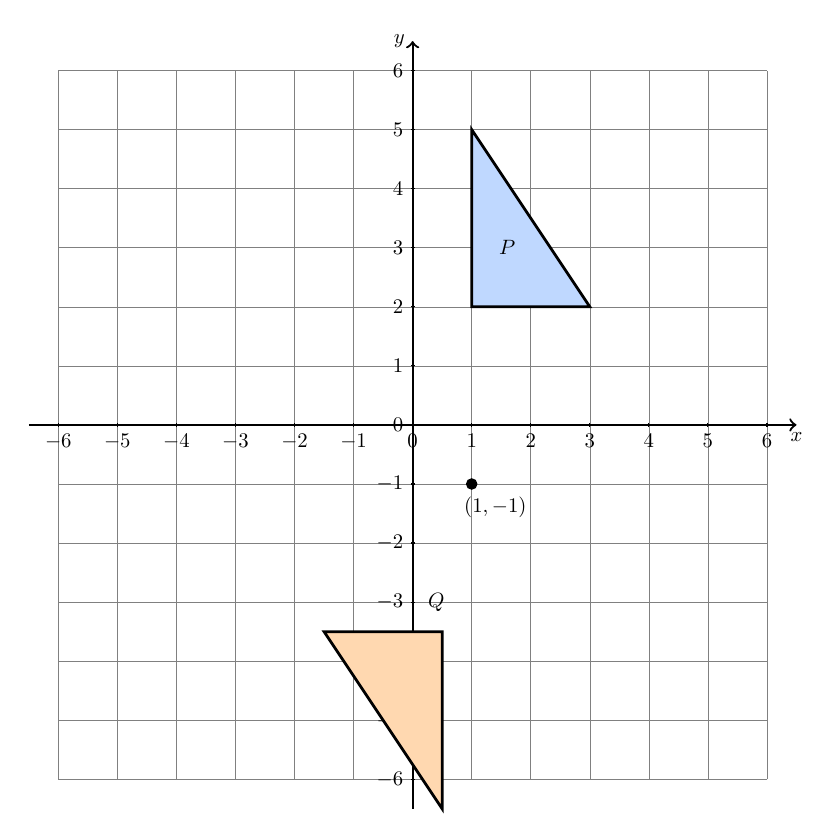
\begin{tikzpicture}[scale=0.75, transform shape]
    % Define axis scale
    \def\axisLimit{6}

    \definecolor{borderColour}{HTML}{000000}
    \definecolor{fillColourP}{HTML}{BFD8FF}
    \definecolor{fillColourQ}{HTML}{FFD8B0}

    % Draw grid
    \draw[step=1cm,gray,very thin] (-\axisLimit,-\axisLimit) grid (\axisLimit,\axisLimit);

    % Draw axes
    \draw[thick,->] (-\axisLimit-0.5,0) -- (\axisLimit+0.5,0) node[anchor=north] {$x$};
    \draw[thick,->] (0,-\axisLimit-0.5) -- (0,\axisLimit+0.5) node[anchor=east] {$y$};

    % Label x-axis and y-axis
    \foreach \x in {-\axisLimit,...,\axisLimit}
        \draw (\x cm,1pt) -- (\x cm,-1pt) node[anchor=north] {$\x$};
    \foreach \y in {-\axisLimit,...,\axisLimit}
        \draw (1pt,\y cm) -- (-1pt,\y cm) node[anchor=east] {$\y$};

    % Triangle P: A(1,2), B(1,5), C(3,2)
    \coordinate (A) at (1,2);
    \coordinate (B) at (1,5);
    \coordinate (C) at (3,2);

    \filldraw[fill=fillColourP, draw=borderColour, line width=1pt] (A) -- (B) -- (C) -- cycle;
    \node at (1.6,3) {$P$};

    % Centre of rotation at (1,-1)
    \coordinate (centre) at (1,-1);
    \filldraw (centre) circle (2.5pt);
    \node at (1.4,-1.4) {$(1,-1)$};

    % Triangle Q: rotate P by 180 degrees about (1,-1)
    % A'(1,-4), B'(1,-7)... need to check within grid; use rotation 180 about (1,-1)
    \coordinate (Ap) at ([rotate around={180:(centre)}]A);
    \coordinate (Bp) at ([rotate around={180:(centre)}]B);
    \coordinate (Cp) at ([rotate around={180:(centre)}]C);

    \filldraw[fill=fillColourQ, draw=borderColour, line width=1pt] (Ap) -- (Bp) -- (Cp) -- cycle;
    \node at (0.4,-3) {$Q$};

\end{tikzpicture}
\end{center}

\noindent Find the transformation that maps triangle $P$ onto triangle $Q$.\\
You must give \textbf{full details} of the transformation.
\vspace{4cm}
\answerlines{3}{3}
\end{question}
